\documentclass[brazil,]{article}
\usepackage{lmodern}
\usepackage{amssymb,amsmath}
\usepackage{ifxetex,ifluatex}
\usepackage{fixltx2e} % provides \textsubscript
\ifnum 0\ifxetex 1\fi\ifluatex 1\fi=0 % if pdftex
  \usepackage[T1]{fontenc}
  \usepackage[utf8]{inputenc}
\else % if luatex or xelatex
  \ifxetex
    \usepackage{mathspec}
  \else
    \usepackage{fontspec}
  \fi
  \defaultfontfeatures{Ligatures=TeX,Scale=MatchLowercase}
  \newcommand{\euro}{€}
\fi
% use upquote if available, for straight quotes in verbatim environments
\IfFileExists{upquote.sty}{\usepackage{upquote}}{}
% use microtype if available
\IfFileExists{microtype.sty}{%
\usepackage{microtype}
\UseMicrotypeSet[protrusion]{basicmath} % disable protrusion for tt fonts
}{}
\usepackage{hyperref}
\PassOptionsToPackage{usenames,dvipsnames}{color} % color is loaded by hyperref
\hypersetup{unicode=true,
            pdftitle={Notas de Aula - Inteligência Artificial},
            pdfauthor={Yuri Malheiros},
            pdfborder={0 0 0},
            breaklinks=true}
\urlstyle{same}  % don't use monospace font for urls
\ifnum 0\ifxetex 1\fi\ifluatex 1\fi=0 % if pdftex
  \usepackage[shorthands=off,main=brazil]{babel}
\else
  \usepackage{polyglossia}
  \setmainlanguage[]{brazil}
\fi



\usepackage{color}
\usepackage{fancyvrb}
\newcommand{\VerbBar}{|}
\newcommand{\VERB}{\Verb[commandchars=\\\{\}]}
\DefineVerbatimEnvironment{Highlighting}{Verbatim}{commandchars=\\\{\}}
% Add ',fontsize=\small' for more characters per line
\usepackage{framed}
\definecolor{shadecolor}{RGB}{248,248,248}
\newenvironment{Shaded}{\begin{snugshade}}{\end{snugshade}}
\newcommand{\KeywordTok}[1]{\textcolor[rgb]{0.13,0.29,0.53}{\textbf{#1}}}
\newcommand{\DataTypeTok}[1]{\textcolor[rgb]{0.13,0.29,0.53}{#1}}
\newcommand{\DecValTok}[1]{\textcolor[rgb]{0.00,0.00,0.81}{#1}}
\newcommand{\BaseNTok}[1]{\textcolor[rgb]{0.00,0.00,0.81}{#1}}
\newcommand{\FloatTok}[1]{\textcolor[rgb]{0.00,0.00,0.81}{#1}}
\newcommand{\ConstantTok}[1]{\textcolor[rgb]{0.00,0.00,0.00}{#1}}
\newcommand{\CharTok}[1]{\textcolor[rgb]{0.31,0.60,0.02}{#1}}
\newcommand{\SpecialCharTok}[1]{\textcolor[rgb]{0.00,0.00,0.00}{#1}}
\newcommand{\StringTok}[1]{\textcolor[rgb]{0.31,0.60,0.02}{#1}}
\newcommand{\VerbatimStringTok}[1]{\textcolor[rgb]{0.31,0.60,0.02}{#1}}
\newcommand{\SpecialStringTok}[1]{\textcolor[rgb]{0.31,0.60,0.02}{#1}}
\newcommand{\ImportTok}[1]{#1}
\newcommand{\CommentTok}[1]{\textcolor[rgb]{0.56,0.35,0.01}{\textit{#1}}}
\newcommand{\DocumentationTok}[1]{\textcolor[rgb]{0.56,0.35,0.01}{\textbf{\textit{#1}}}}
\newcommand{\AnnotationTok}[1]{\textcolor[rgb]{0.56,0.35,0.01}{\textbf{\textit{#1}}}}
\newcommand{\CommentVarTok}[1]{\textcolor[rgb]{0.56,0.35,0.01}{\textbf{\textit{#1}}}}
\newcommand{\OtherTok}[1]{\textcolor[rgb]{0.56,0.35,0.01}{#1}}
\newcommand{\FunctionTok}[1]{\textcolor[rgb]{0.00,0.00,0.00}{#1}}
\newcommand{\VariableTok}[1]{\textcolor[rgb]{0.00,0.00,0.00}{#1}}
\newcommand{\ControlFlowTok}[1]{\textcolor[rgb]{0.13,0.29,0.53}{\textbf{#1}}}
\newcommand{\OperatorTok}[1]{\textcolor[rgb]{0.81,0.36,0.00}{\textbf{#1}}}
\newcommand{\BuiltInTok}[1]{#1}
\newcommand{\ExtensionTok}[1]{#1}
\newcommand{\PreprocessorTok}[1]{\textcolor[rgb]{0.56,0.35,0.01}{\textit{#1}}}
\newcommand{\AttributeTok}[1]{\textcolor[rgb]{0.77,0.63,0.00}{#1}}
\newcommand{\RegionMarkerTok}[1]{#1}
\newcommand{\InformationTok}[1]{\textcolor[rgb]{0.56,0.35,0.01}{\textbf{\textit{#1}}}}
\newcommand{\WarningTok}[1]{\textcolor[rgb]{0.56,0.35,0.01}{\textbf{\textit{#1}}}}
\newcommand{\AlertTok}[1]{\textcolor[rgb]{0.94,0.16,0.16}{#1}}
\newcommand{\ErrorTok}[1]{\textcolor[rgb]{0.64,0.00,0.00}{\textbf{#1}}}
\newcommand{\NormalTok}[1]{#1}
\DefineVerbatimEnvironment{Highlighting}{Verbatim}{commandchars=\\\{\},fontsize=\small}

\usepackage{graphicx,grffile}
\makeatletter
\def\maxwidth{\ifdim\Gin@nat@width>\linewidth\linewidth\else\Gin@nat@width\fi}
\def\maxheight{\ifdim\Gin@nat@height>\textheight\textheight\else\Gin@nat@height\fi}
\makeatother
% Scale images if necessary, so that they will not overflow the page
% margins by default, and it is still possible to overwrite the defaults
% using explicit options in \includegraphics[width, height, ...]{}
\setkeys{Gin}{width=\maxwidth,height=\maxheight,keepaspectratio}
\setlength{\parindent}{0pt}
\setlength{\parskip}{6pt plus 2pt minus 1pt}
\setlength{\emergencystretch}{3em}  % prevent overfull lines
\providecommand{\tightlist}{%
  \setlength{\itemsep}{0pt}\setlength{\parskip}{0pt}}
\setcounter{secnumdepth}{0}

% Overwrite \begin{figure}[htbp] with \begin{figure}[H]
\usepackage{float}
\let\origfigure=\figure
\let\endorigfigure=\endfigure
\renewenvironment{figure}[1][]{%
\origfigure[H]
}{%
\endorigfigure
}

\title{Notas de Aula - Inteligência Artificial}
\author{Yuri Malheiros}
\date{UFPB - Campus IV - Rio Tinto}

% Redefines (sub)paragraphs to behave more like sections
\ifx\paragraph\undefined\else
\let\oldparagraph\paragraph
\renewcommand{\paragraph}[1]{\oldparagraph{#1}\mbox{}}
\fi
\ifx\subparagraph\undefined\else
\let\oldsubparagraph\subparagraph
\renewcommand{\subparagraph}[1]{\oldsubparagraph{#1}\mbox{}}
\fi

\begin{document}
\maketitle

\section{Resolução de problemas}\label{resoluuxe7uxe3o-de-problemas}

\subsection{1. Introdução}\label{introduuxe7uxe3o}

Uma das formas mais simples de resolver um problema é executar uma
sequência de passos para sair de um estado inicial, no qual o problema
não está resolvido, até um objetivo, isto é, um estado no qual o
problema está resolvido.

O processo de procurar uma solução de um problema através da exploração
sistemática dos seus possíveis estados é chamado de \textbf{busca}. Como
solução, a busca encontra uma sequência fixa de ações para sair do
estado inicial e chegar no objetivo. É importante ressaltar, que nessa
abordagem não existe um plano alternativo se algo der errado durante a
execução da solução.

Este problema pode ser entendido como um problema de encontrar um
caminho num grafo, que começa no estado inicial e termina no objetivo.

Para utilizar uma busca para resolver um problema, o ambiente que o
agente inteligente está inserido deve ser: observável, discreto e
determinístico.

A Figura 1 apresenta um mapa com algumas cidades do estado da Paraíba.
Nele, uma busca pode ser usada para encontrar um caminho, por exemplo,
da cidade João Pessoa até a cidade Cajazeiras, como é mostrado na Figura
2.

\begin{figure}
\centering
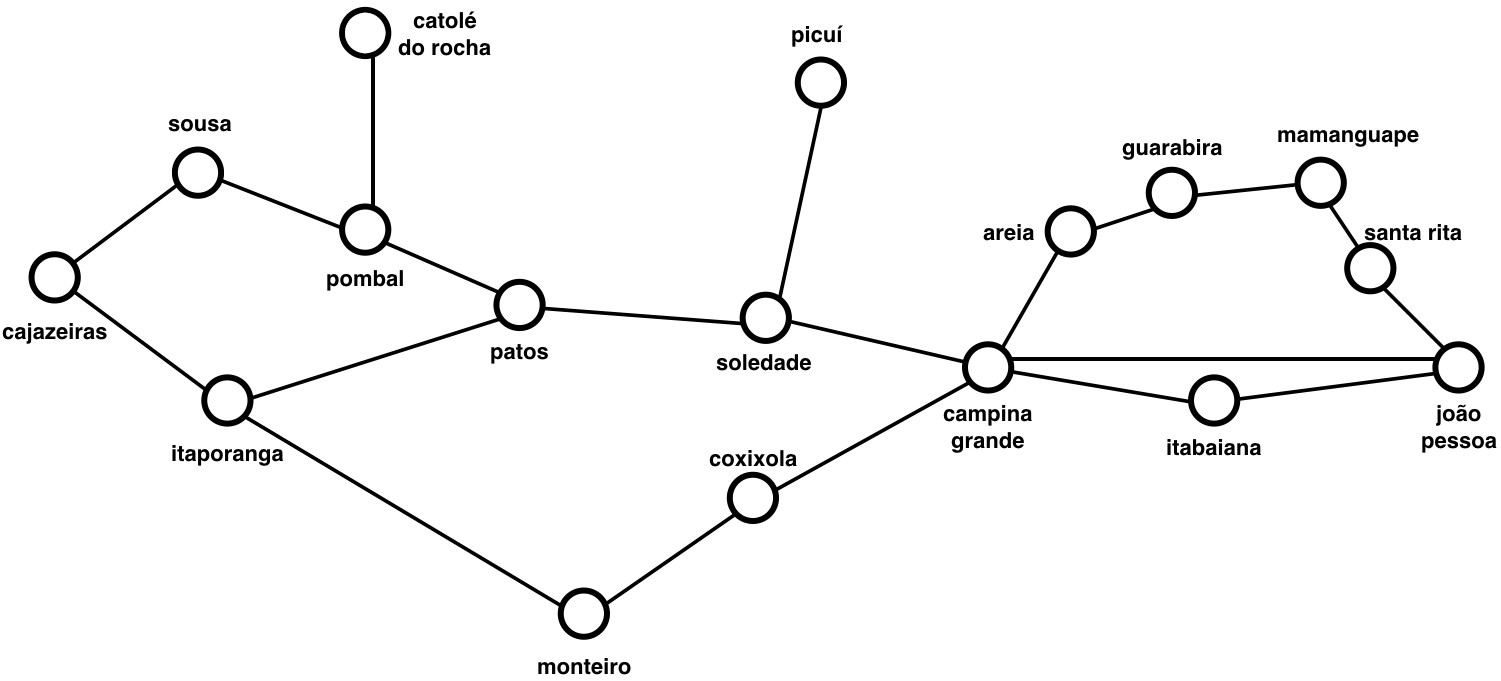
\includegraphics{pbmapa.png}
\caption{Mapa simplificado da Paraíba.}
\end{figure}

\begin{figure}
\centering
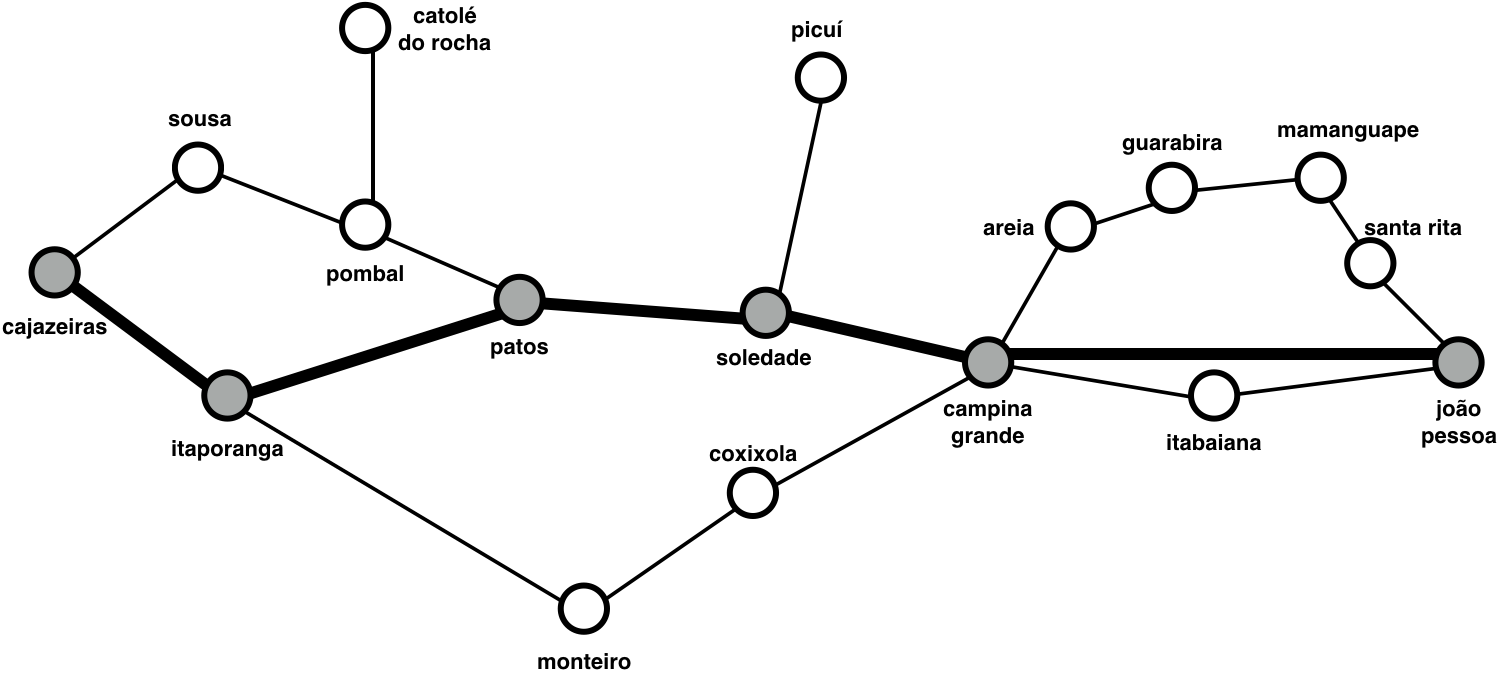
\includegraphics{pbmapa-solucao.png}
\caption{Caminho entre a cidade João Pessoa e Cajazeiras.}
\end{figure}

\subsection{2. Formulando problemas}\label{formulando-problemas}

Um problema de busca pode ser definido por 6 componentes:

\begin{itemize}
\tightlist
\item
  Estado inicial: estado onde o agente começa;
\item
  Ações(s): função que retorna as possíveis ações dado um estado
  \emph{s};
\item
  Resultado(s, a): retorna o estado resultante da ação \emph{a} a partir
  do estado \emph{s};
\item
  Objetivo(s): testa se \emph{s} é um objetivo ou não;
\item
  Custo(s, a, s'): custo para executar a ação \emph{a} a partir de
  \emph{s} para chegar em \emph{s'};
\item
  Objetivos: estados que solucionam o problema.
\end{itemize}

\subsection{3. Busca genérica em
grafo}\label{busca-genuxe9rica-em-grafo}

Veremos mais a frente diversos tipos de buscas em grafos, entretanto
todas essas buscas compartilham uma mesma base. Assim, primeiramente
apresentaremos um algoritmo genérico de busca em grafo, que será
transformado mais a frente em tipos específicos de busca.

A ideia do algoritmo de busca em grafo é sair do estado inicial para
encontrar o objetivo explorando caminhos iterativamente. Usando o mapa
da Figura 1, dado que seu estado inicial é a cidade João Pessoa, o
algoritmo inicia verificando quais as ações possíveis a partir de João
Pessoa. Nesse caso, o agente poderia ir para as cidades Santa Rita,
Campina Grande ou Itabaiana (Figura 3a). Esses três estados formam um
conjunto de estados que podem ser explorados a partir do estado atual,
no algoritmo, ele recebe o nome de \textbf{borda} (ou fronteira). Uma
decisão fundamental no algoritmo é a estratégia de escolha do estado da
borda que será explorado, diferentes estratégias podem resultar em
diferentes algoritmos de busca.

Continuando a exploração, se Campina Grande for escolhida, então o
algoritmo retira Campina Grande da borda e adiciona os estados que podem
ser alcançados a partir dela, fazendo com que a borda agora possua os
nós: Santa Rita, Itabaiana, Areia, Soledade e Coxixola (Figura 3b). É
importante perceber, que de Campina Grande também é possível chegar em
Itabaiana, mas esse estado já estava na borda. Um algoritmo de busca em
grafo descarta estados repetidos, então Itabaiana não deve ser
adicionada à borda novamente.

\begin{figure}
\centering
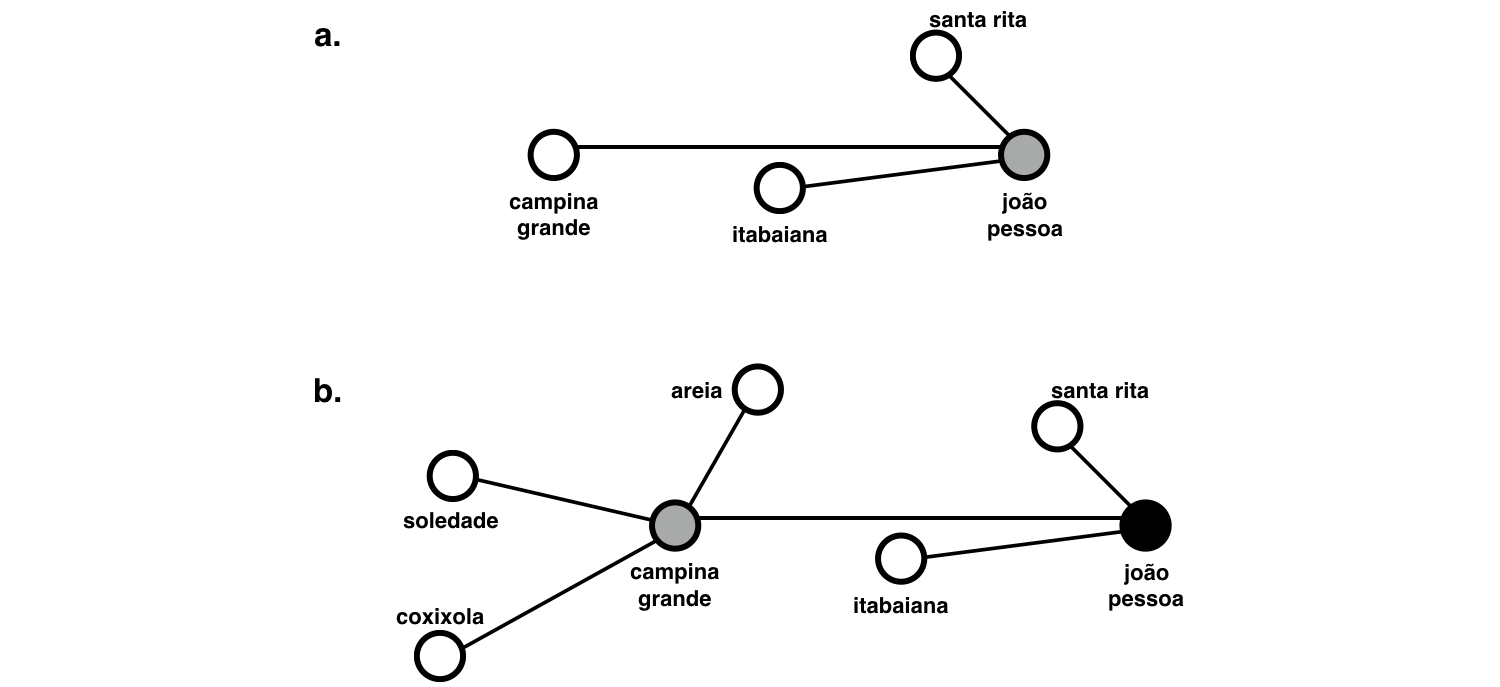
\includegraphics{pbmapa-algoritmo.png}
\caption{a) Estado inicial João Pessoa e os estados acessíveis a partir
dele formando a borda. b) Estado Campina Grande explorado, estado João
Pessoa já visitado e os estados restantes formando a borda.}
\end{figure}

Esse processo se repete até que o estado explorado seja um objetivo ou
até que a borda seja vazia, nesse último caso, temos que não foi
possível alcançar o objetivo.

O algoritmo a seguir implementa em Python a busca genérica em grafo:

\hypertarget{mycode}{\label{mycode}}
\begin{Shaded}
\begin{Highlighting}[numbers=left,,]
\KeywordTok{def}\NormalTok{ generic_search():}
\NormalTok{    frontier }\OperatorTok{=}\NormalTok{ [initial_state]}
\NormalTok{    explored }\OperatorTok{=} \BuiltInTok{set}\NormalTok{()}

    \ControlFlowTok{while} \VariableTok{True}\NormalTok{:}
        \ControlFlowTok{if} \BuiltInTok{len}\NormalTok{(frontier) }\OperatorTok{==} \DecValTok{0}\NormalTok{:}
            \ControlFlowTok{return} \VariableTok{False}

\NormalTok{        new_state }\OperatorTok{=}\NormalTok{ choose_state(frontier)}
\NormalTok{        explored.add(new_state)}

        \ControlFlowTok{if}\NormalTok{ new_state }\KeywordTok{in}\NormalTok{ goals:}
            \ControlFlowTok{return}\NormalTok{ new_state}

        \ControlFlowTok{for}\NormalTok{ state }\KeywordTok{in}\NormalTok{ new_state.actions:}
            \ControlFlowTok{if}\NormalTok{ state }\KeywordTok{not} \KeywordTok{in}\NormalTok{ explored }\KeywordTok{or}\NormalTok{ state }\KeywordTok{not} \KeywordTok{in}\NormalTok{ frontier:}
\NormalTok{                frontier.append(state)}
\end{Highlighting}
\end{Shaded}

Na linha 2, o algoritmo inicializa a borda com o estado inicial, em
seguida, na linha 5, ele entre num loop até que atinja uma das condições
de parada. Na linha 9 é feita a escolha de um estado na borda, a função
\emph{choose\_state} deve ser implementada de acordo com a estratégia de
escolha dos estados na borda. O for na linha 15 serve para adicionar à
borda os estados que podem ser alcançados através das possíveis ações
executadas em \emph{new\_state}. As linhas 3, 10 e 16 são responsáveis
por evitar que estados redundantes sejam adicionados à borda. Na linha 3
um set que guardará os estados explorados é iniciado, na linha 10 o
estado explorado é adicionado ao set e na linha 16 temos uma condição
para que apenas um estado que não esteja no set ou não esteja na borda
seja adicionado à borda.

Na implementação, é importante deixar clara a diferença entre os estados
de um problema e os nós no grafo onde a busca é realizada. Até aqui, os
conceitos foram utilizados sem distinção, mas, para implementar as
buscas, precisamos deixar claro o papel de cada um.

Um estado corresponde a uma configuração de mundo, ou seja, a um estado
do problema. Um nó é uma estrutura do grafo, que contém um estado, o
custo para se chegar até esse estado e uma referência para o estado pai,
isto é, o estado anterior no qual foi executado uma ação para se chegar
ao estado do nó. Ao final da busca, as referências para o estado pai
podem ser utilizadas para recuperar o caminho percorrido do estado
inicial até o objetivo. Por fim, é importante saber que dois nós
distintos, podem conter o mesmo estado, isso acontece quando caminhos
diferentes no grafo levam a um mesmo estado.

\subsection{4. Busca sem informações (busca
cega)}\label{busca-sem-informauxe7uxf5es-busca-cega}

Os primeiros algoritmos de busca que serão abordados são algoritmos de
busca sem informações (ou busca cega). Estes algoritmos recebem tal
nome, pois seus estados não possuem informação relacionada a sua
qualidade em relação ao objetivo. Ou seja, ao escolher um estado, o
algoritmo não tem ideia do custo desse estado até o objetivo. Por
exemplo, num problema para encontrar um caminho entre duas cidades, não
se tem a informação se uma cidade está mais próxima do objetivo do que
outra.

A seguir veremos três tipos de buscas: busca em largura, busca de custo
uniforme e busca em profundidade.

\subsubsection{4.1. Busca em largura}\label{busca-em-largura}

A busca em largura é uma estratégia de busca simples, na qual o nó
inicial é explorado, em seguida os sucessores do nó inicial são
explorados, depois os sucessores desses nós, etc. Nesse caso, a
estratégia de escolha de um nó na borda é simplemente explorar o nó que
foi adicionado primeiramente à borda, ou seja, a borda funciona como uma
fila. Dada a árvore da Figura 4, a ordem de visitação dos nós aplicando
a busca em largura com estado inicial A e objetivo G é: A, B, C, D, E, F
e G.

\begin{figure}
\centering
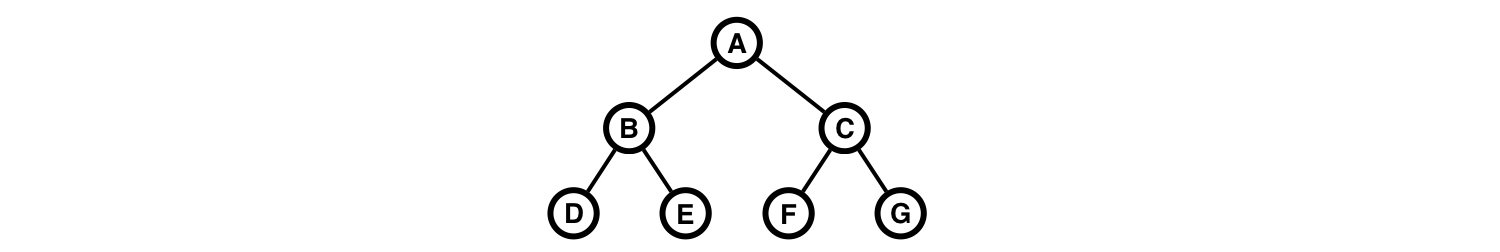
\includegraphics{arvore.png}
\caption{Árvore binária.}
\end{figure}

O algoritmo de busca em largura é completo, isto é, ele sempre encontra
a solução se ela existir. Além disso, ele é ótimo se os custos dos
caminhos forem iguais. As complexidades de tempo e espaço são as mesmas,
\(\mathcal{O}(b^d)\), onde \(b\) é o número de sucessores de um nó e
\(d\) é a profundidade onde se encontra o objetivo. A complexidade
exponencial é uma característica muito ruim desse tipo de busca. Num
problema com \(b=10\) e \(d=2\), se cada nó for representado por 1kb, o
algoritmo usará 100kb de memória, se aumentarmos d para 4, esse valor
passa para 10mb, se dobrarmos d novamente, ou seja, tivermos um problema
onde o objetivo se encontra no 8° nível de profundidade, o algoritmo
usará cerca de 100gb!

\subsubsection{4.2. Busca de custo
uniforme}\label{busca-de-custo-uniforme}

A busca de custo uniforme é uma extensão da busca em largura, que é
ótima mesmo quando existirem caminhos com custos diferentes. Nela, ao
invés de escolher o primeiro nó de uma fila que representa a borda,
expande-se o nó com o menor custo de caminho (\(g(s)\)). Para isso,
basta representar a borda como uma fila de prioridade, na qual o nó com
menor \(g(s)\) tem a maior prioridade. É importante observar que o custo
de caminho \(g(s)\), não é apenas o custo do \emph{pai de s} até
\emph{s}, mas sim o custo do estado inicial até s.

Para implementação, existe uma modificação importante a ser feita no
algoritmo de busca genérica apresentado anteriormente. Quando um nó já
estiver na fronteira e o algoritmo tentar adicionar ele novamente, é
necessário verificar se esse novo caminho para o nó tem um custo menor
que o custo de caminho do nó na fronteira, se isso for verdade, o nó
deve ser substituído.

No grafo da Figura 5, se for usada a busca de custo uniforme para sair
de A até encontrar o objetivo E, os seguintes passos vão ocorrer.
Primeiro explora-se o estado inicial A, com isso tem-se dois nós na
borda: B e C. Como B tem o menor custo (10), então ele é escolhido,
adicionando o nó D com custo 40 (10+30) à borda. O próximo nó explorado
será C, que tem custo 20, assim o nó E será adicionado à borda com custo
120 (20+100). A seguir, o nó D é explorado e novamente tem-se o nó E
para ser adicionado à borda. Nesse caso, o caminho para E tem custo 80
(10+30+40), que é menor que custo de chegar em E através de D (120).
Assim, o algoritmo substitui o nó E na borda, pelo nó com o menor custo.

\begin{figure}
\centering
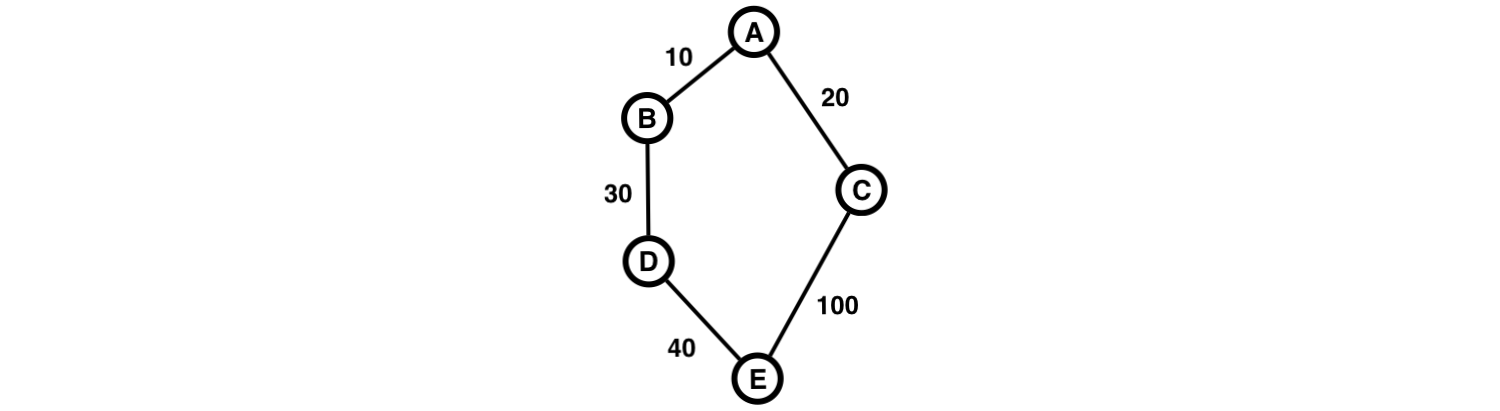
\includegraphics{grafo.png}
\caption{Grafo para ilustrar a troca de nós na borda numa busca de custo
uniforme.}
\end{figure}

Dada a árvore da Figura 6, a ordem de visitação dos nós aplicando a
busca de custo uniforme com estado inicial A e objetivo G é: A, B, C, F,
D, G.

\begin{figure}
\centering
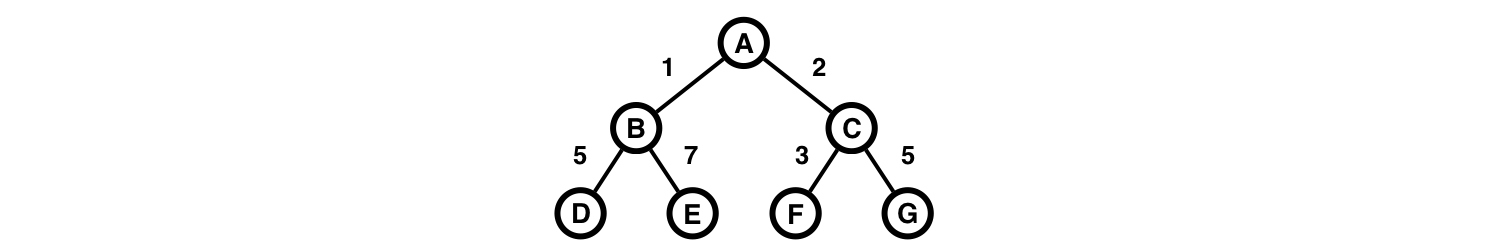
\includegraphics{arvore-custos.png}
\caption{Árvore com custos.}
\end{figure}

A busca de custo uniforme é completa. Ela também é ótima se todos os
custos do problema forem não negativos. Assim como a busca em largura, a
busca de custo uniforme possui complexidade de tempo e espaço
exponenciais.

\subsubsection{4.3. Busca em profundidade}\label{busca-em-profundidade}

Na busca em profundidade, a estratégia de escolha de um estado na borda
é selecionar o último estado que foi adicionado. Assim, a borda nesse
algoritmo pode ser representada por uma pilha. Dada a árvore da Figura
4, a ordem de visitação dos nós aplicando a busca em largura com estado
inicial A e objetivo G é: A, B, D, E, C, F, G.

O algoritmo de busca em profundidade é completo, porém ele não é ótimo.
Suponha que na Figura 4 o nó D seja um objetivo e C também. Nesse caso,
a busca em profundidade retornaria D como solução, mesmo C sendo uma
solução melhor. A complexidade temporal é \(\mathcal{O}(b^m)\), onde m é
a profundidade máxima. Já a complexidade espacial é \(\mathcal{O}(bm)\),
o que faz o uso de memória desse algoritmo ser muito menor que o da
busca em largura e da busca em custo uniforme. Isso é possível, porque
após um nó e todos os seus descendentes serem visitados, eles podem ser
removidos da memória sem comprometer o funcionamento do algoritmo.

\subsection{5. Busca informada (busca
heurística)}\label{busca-informada-busca-heuruxedstica}

Nas buscas apresentadas na seção anterior, ao explorar os estados de um
problema, não era levado em consideração se ele estava mais perto ou
mais longe da solução. Para resolver isso, a busca informada utiliza
conhecimentos específicos do problema que está sendo resolvido. Nela,
uma \textbf{função heurística} \(h(n)\) é utilizada para ajudar a
decidir que nós são mais promissores para a solução de um problema.

Esse tipo de busca é semelhante a busca de custo uniforme, mas com uma
função de custo diferente, que vai utilizar a função heurística.

No geral, a busca informada pode encontrar soluções de forma mais
eficiente que a busca sem informações.

A seguir veremos dois tipos de buscas: busca gulosa e busca A*.

\subsubsection{5.1. Busca gulosa}\label{busca-gulosa}

Na busca gulosa, também é usada uma fila de prioridade, como na busca de
custo uniforme, para representar a borda. Entretanto, o custo utilizado
é o custo avaliado pela função heurística (\(h(s)\)). Assim, o nó
escolhido na borda será o nó com o menor valor de \(h(s)\), isto é, o nó
que mais se aproxima da solução.

A Figura 7, traz novamente o mapa com algumas cidades da Paraíba, mas
dessa vez acrescido dos custos para ir de uma cidade para outra (os
valores que aparecem nas arestas) e das distâncias em linha reta entre
os estados e o objetivo que é a cidade de Cajazeiras (os valores entre
parênteses próximos aos nomes das cidades). Nesse exemplo usaremos a
distância em linha reta entre um estado e o objetivo como a função
heurística.

\begin{figure}
\centering
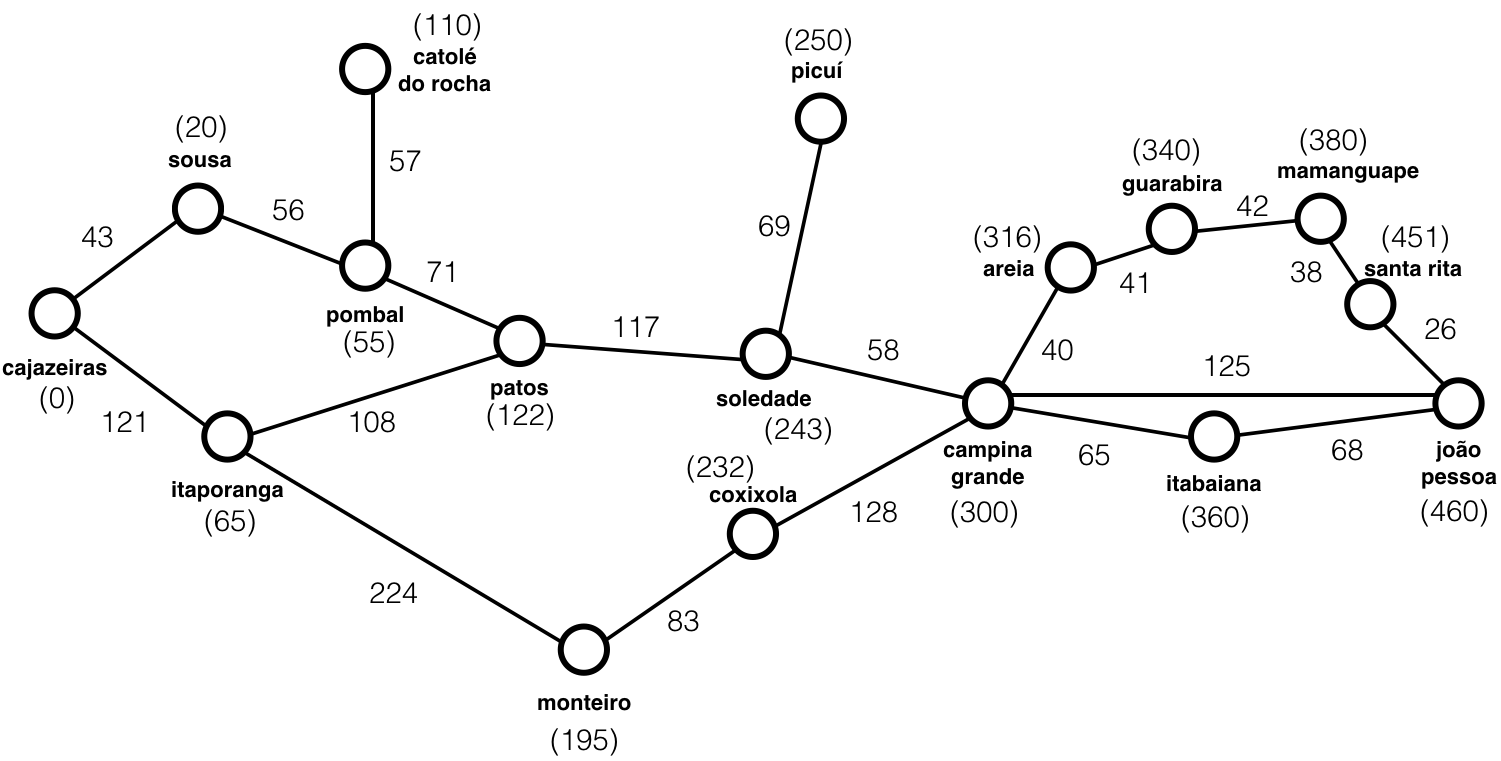
\includegraphics{pbmapa-custos-estimativa.png}
\caption{Mapa simplificado da Paraíba com custos entre as cidades e a
distância em linha reta entre cada cidade e Cajazeiras.}
\end{figure}

Dado que o estado inicial é João Pessoa, a seguir tem-se uma lista das
fronteiras e dos nós escolhidos em cada iteração do algoritmo:

\begin{verbatim}
Iteração 1
Fronteira: [João Pessoa (460)]
Nó escolhido: João Pessoa

Iteração 2
Fronteira: [Santa Rita (451), Campina Grande (300), Itabaiana (360)]
Nó escolhido: Campina Grande

Iteração 3
Fronteira: [Santa Rita (451), Itabaiana (360), Areia (316),
            Soledade (243), Coxixola (232)]
Nó escolhido: Coxixola

Iteração 4
Fronteira: [Santa Rita (451), Itabaiana (360), Areia (316),
            Soledade (243), Monteiro (195)]
Nó escolhido: Monteiro

Iteração 5
Fronteira: [Santa Rita (451), Itabaiana (360), Areia (316),
            Soledade (243), Itaporanga (65)]
Nó escolhido: Itaporanga

Iteração 6
Fronteira: [Santa Rita (451), Itabaiana (360), Areia (316),
            Soledade (243), Patos(122), Cajazeiras (0)]
Nó escolhido: Cajazeiras

Solução: João Pessoa, Campina Grande, Coxixola, Monteiro,
         Itaporanga, Cajazeiras.
\end{verbatim}

A busca gulosa é completa, mas não é ótima. Note que no exemplo
anterior, o caminho encontrado possui custo 701, entretanto o caminho
João Pessoa, Campina Grande, Soledade, Patos, Pombal, Sousa, Cajazeiras
tem custo 470. No pior caso, a complexidade de tempo e espaço é
\(\mathcal{O}(b^m)\), onde m é a profundidade máxima. No entanto,
dependendo do problema e da função heurística utilizada, a complexidade
é reduzida substancialmente.

\subsubsection{5.2. Busca A*}\label{busca-a}

A busca A* une os conceitos da busca gulosa e da busca de custo
uniforme, assim, sua borda é uma fila de prioridade, na qual o custo
associado a um estado é \(f(s) = h(s) + g(s)\), onde \(h(s)\) é a função
heurística e \(g(s)\) o custo de caminho.

Usando o exemplo da Figura 7 com estado inicial João Pessoa e objetivo
Cajazeiras e mais uma vez com \(h(s)\) sendo a distância em linha reta
entre um estado e o objetivo, a seguir é mostrada uma lista das
fronteiras e dos nós escolhidos em cada iteração do algoritmo:

\begin{Shaded}
\begin{Highlighting}[]
\NormalTok{Iteração 1}
\NormalTok{Fronteira: [João Pessoa (460+0 = 460)]}
\NormalTok{Nó escolhido: João Pessoa}

\NormalTok{Iteração 2}
\NormalTok{Fronteira: [Santa Rita (451+26 = 477), Campina Grande (300+125 = 425),}
\NormalTok{            Itabaiana (360+68 = 428)]}
\NormalTok{Nó escolhido: Campina Grande}

\NormalTok{Iteração 3}
\NormalTok{Fronteira: [Santa Rita (451+26 = 477), Itabaiana (360+68 = 428),}
\NormalTok{            Areia (316+165 = 481), Soledade (243+183 = 426),}
\NormalTok{            Coxixola (232+253 = 485)]}
\NormalTok{Nó escolhido: Soledade}

\NormalTok{Iteração 4}
\NormalTok{Fronteira: [Santa Rita (451+26 = 477), Itabaiana (360+68 = 428),}
\NormalTok{            Areia (316+165 = 481), Coxixola (232+253 = 485),}
\NormalTok{            Picuí (250+252 = 502), Patos (122+300 = 422)]}
\NormalTok{Nó escolhido: Patos}

\NormalTok{Iteração 5}
\NormalTok{Fronteira: [Santa Rita (45)+26 = 477), Itabaiana (360+68 = 428),}
\NormalTok{            Areia (316+165 = 481), Coxixola (232+253 = 485),}
\NormalTok{            Picuí (250+252 = 502), Pombal (55+371 = 426),}
\NormalTok{            Itaporanga (65+408 = 473)]}
\NormalTok{Nó escolhido: Pombal}

\NormalTok{Iteração 6}
\NormalTok{Fronteira: [Santa Rita (451+26 = 477), Itabaiana (360+68 = 428),}
\NormalTok{            Areia (316+165 = 481), Coxixola (232+253 = 485),}
\NormalTok{            Picuí (250+252 = 502), Itaporanga (65+408 = 473),}
\NormalTok{            Sousa (20+427 = 447), Catolé do Rocha (110+428 = 538)]}
\NormalTok{Nó escolhido: Itabaiana}

\NormalTok{Iteração 7}
\NormalTok{Fronteira: [Santa Rita (451+26 = 477), Areia (316+165 = 481),}
\NormalTok{            Coxixola (232+253 = 485), Picuí (250+252 = 502),}
\NormalTok{            Itaporanga (65+408 = 473), Sousa (20+427 = 447),}
\NormalTok{            Catolé do Rocha (110+428 = 538)]}
\NormalTok{Nó escolhido: Sousa}

\NormalTok{Iteração 8}
\NormalTok{Fronteira: [Santa Rita (451+26 = 477), Areia (316+165 = 481),}
\NormalTok{            Coxixola (232+253 = 485), Picuí (250+252 = 502),}
\NormalTok{            Itaporanga (65+408 = 473), Catolé do Rocha (110+428 = 538),}
\NormalTok{            Cajazeiras (0+470 = 470)]}
\NormalTok{Nó escolhido: Cajazeiras}

\NormalTok{Solução: João Pessoa, Campina Grande, Soledade, Patos, Pombal,}
\NormalTok{         Sousa, Cajazeiras.}
\end{Highlighting}
\end{Shaded}

Nesse algoritmo, é importante que a função heurística não superestime o
custo de atingir o objetivo, isto é, \(h(n) < custo real\). Tal
característica é chamada de admissibilidade. Além disso, para o
algoritmo ser ótimo, \(h(n)\) precisa ser consistente, ou seja, \(h(s)\)
precisa ser menor ou igual que o custo de ir do estado \emph{s} para o
seu sucessor \emph{s'} somado com h(s'). Matematicamente a consistência
é definida como: \(h(s) \leq custo(s, a, s') + h(s')\).

A busca A* é completa e ótima se \(h(n)\) for consistente, mas a sua
complexidade continua sendo exponencial no pior caso como em outros
algoritmos. Nessa busca, a memória ocupada é um problema bem maior que o
tempo de execução, mas mesmo assim, uma boa função heurística ainda
fornece uma grande vantagem em relação aos algoritmos de busca sem
informações.

\end{document}
